\documentclass[a4paper, 11pt]{article}
\usepackage{amsmath}
\usepackage{graphicx}
\usepackage{geometry}
\usepackage{listings}
\geometry{scale=0.8}
\linespread{1.5}
\usepackage{hyperref}
\usepackage{listings}


\title{	
\normalfont \normalsize
\textsc{School of Data and Computer Science, Sun Yat-sen University} \\ [25pt] %textsc small capital letters
\rule{\textwidth}{0.5pt} \\[0.4cm] % Thin top horizontal rule
\huge  E09 Variable Elimination \\ % The assignment title
\rule{\textwidth}{2pt} \\[0.5cm] % Thick bottom horizontal rule
\author{20214966 Yangkai Lin 20214810 Suixin Ou}
\date{\normalsize\today}
}

\begin{document}
\maketitle
\tableofcontents
\newpage


\section{VE}

The burglary example is described as following:
\begin{figure}[h]
  \centering

  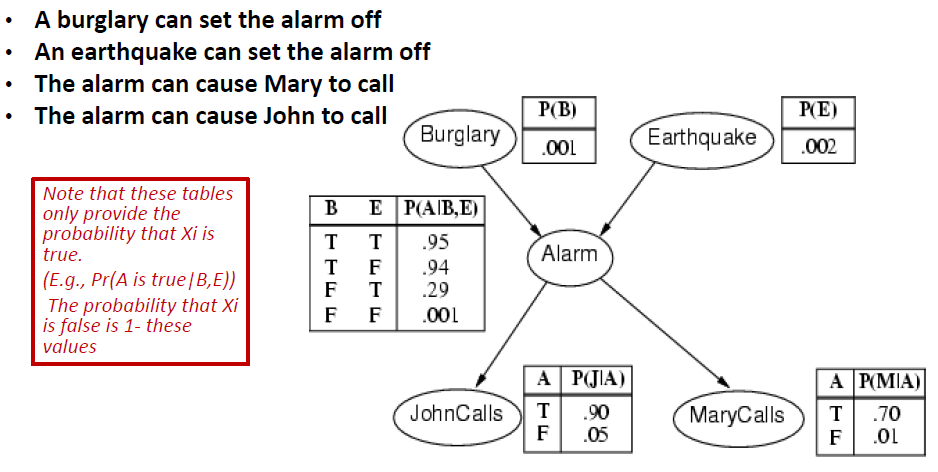
\includegraphics[width=14cm]{Pic/burglary}
\end{figure}

\begin{figure}[ht]
\centering
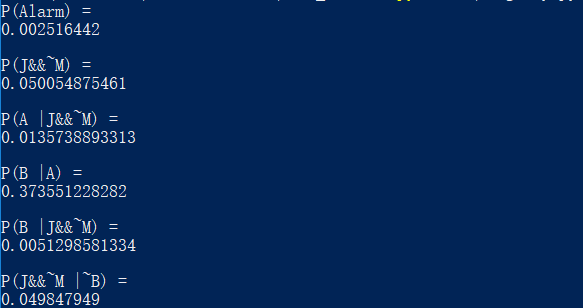
\includegraphics[width=12cm]{Pic/burglar_result}
\end{figure}
Here is a VE template for you to solve the burglary example:
\begin{lstlisting}[language=Python,frame=single]
class VariableElimination:
    @staticmethod
    def inference(factorList, queryVariables, 
    orderedListOfHiddenVariables, evidenceList):
        for ev in evidenceList:
            #Your code here
        for var in orderedListOfHiddenVariables:
            #Your code here
        print "RESULT:"
        res = factorList[0]
        for factor in factorList[1:]:
            res = res.multiply(factor)
        total = sum(res.cpt.values())
        res.cpt = {k: v/total for k, v in res.cpt.items()}
        res.printInf()
    @staticmethod
    def printFactors(factorList):
        for factor in factorList:
            factor.printInf()
class Util:
    @staticmethod
    def to_binary(num, len):
        return format(num, '0' + str(len) + 'b')
class Node:
    def __init__(self, name, var_list):
        self.name = name
        self.varList = var_list
        self.cpt = {}
    def setCpt(self, cpt):
        self.cpt = cpt
    def printInf(self):
        print "Name = " + self.name
        print " vars " + str(self.varList)
        for key in self.cpt:
            print "   key: " + key + " val : " + str(self.cpt[key])
        print ""
    def multiply(self, factor):
        """function that multiplies with another factor"""
        #Your code here
        new_node = Node("f" + str(newList), newList)
        new_node.setCpt(new_cpt)
        return new_node
    def sumout(self, variable):
        """function that sums out a variable given a factor"""
        #Your code here
        new_node = Node("f" + str(new_var_list), new_var_list)
        new_node.setCpt(new_cpt)
        return new_node
    def restrict(self, variable, value):
        """function that restricts a variable to some value 
        in a given factor"""
        #Your code here
        new_node = Node("f" + str(new_var_list), new_var_list)
        new_node.setCpt(new_cpt)
        return new_node
# create nodes for Bayes Net
B = Node("B", ["B"])
E = Node("E", ["E"])
A = Node("A", ["A", "B","E"])
J = Node("J", ["J", "A"])
M = Node("M", ["M", "A"])

# Generate cpt for each node
B.setCpt({'0': 0.999, '1': 0.001})
E.setCpt({'0': 0.998, '1': 0.002})
A.setCpt({'111': 0.95, '011': 0.05, '110':0.94,'010':0.06,
'101':0.29,'001':0.71,'100':0.001,'000':0.999})
J.setCpt({'11': 0.9, '01': 0.1, '10': 0.05, '00': 0.95})
M.setCpt({'11': 0.7, '01': 0.3, '10': 0.01, '00': 0.99})

print "P(A) **********************"
VariableElimination.inference([B,E,A,J,M], ['A'], ['B', 'E', 'J','M'], {})

print "P(B | J~M) **********************"
VariableElimination.inference([B,E,A,J,M], ['B'], ['E','A'], {'J':1,'M':0})
\end{lstlisting}
\section{Task}
\begin{itemize}
\item You should implement 4 functions: \texttt{inference}, \texttt{multiply}, \texttt{sumout} and \texttt{restrict}. You can turn to Figure \ref{Fig:ve_product} and Figure \ref{Fig:sumout_restrict} for help. 
\item Please hand in a file named \textsf{E09\_YourNumber.pdf}, and send it to \textsf{ai\_2020@foxmail.com}
\end{itemize}


\begin{figure}[ht]{}
\centering
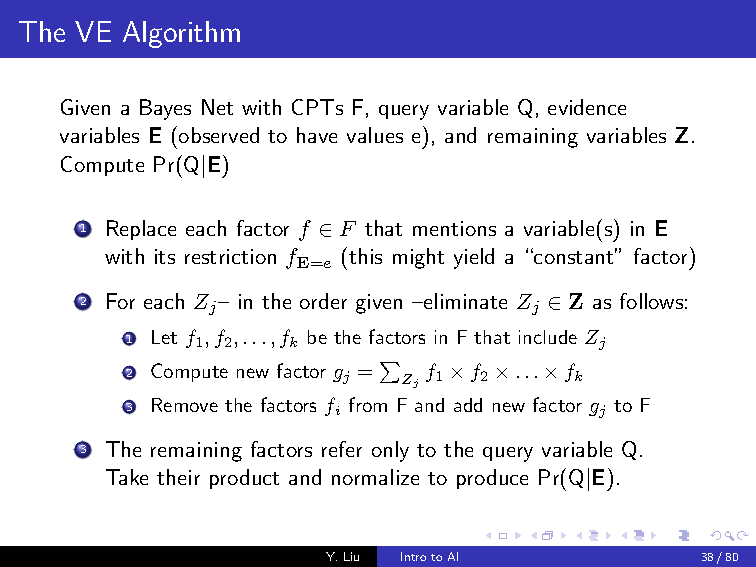
\includegraphics[width=7.5cm]{Pic/ve}
\qquad
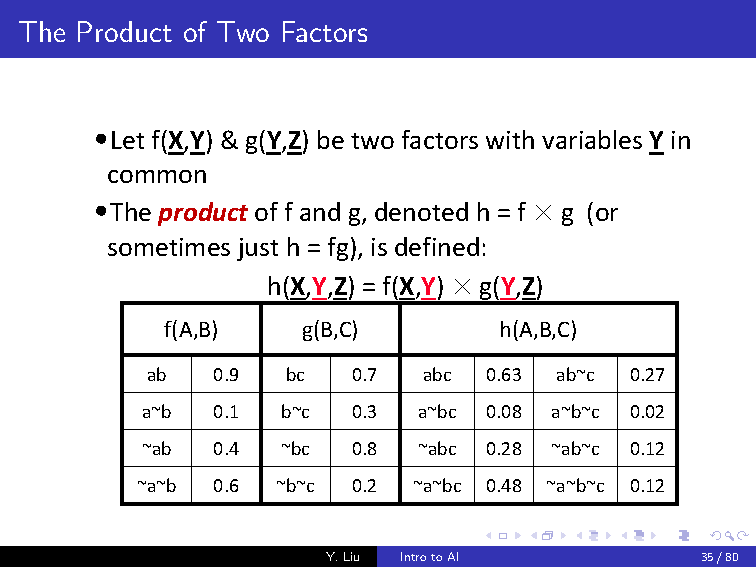
\includegraphics[width=7.5cm]{Pic/product}
\caption{VE and Product}
\label{Fig:ve_product}
\end{figure}


\begin{figure}[ht]
\centering
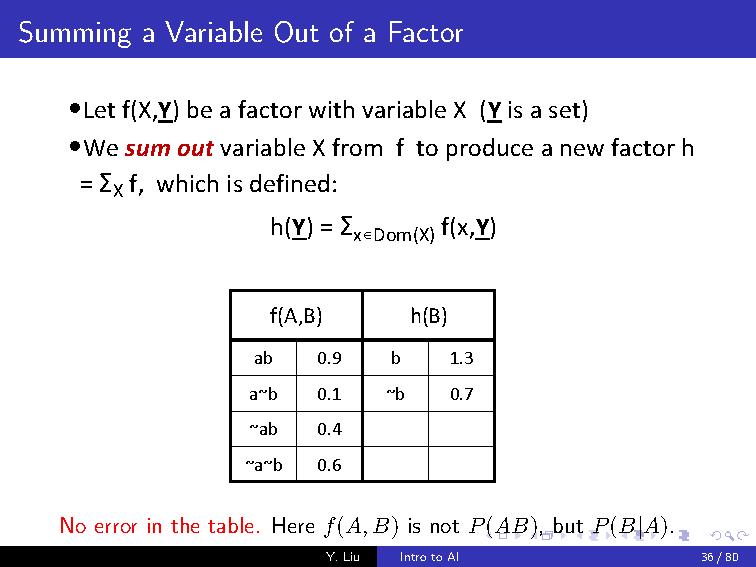
\includegraphics[width=7.5cm]{Pic/sumout}
\qquad
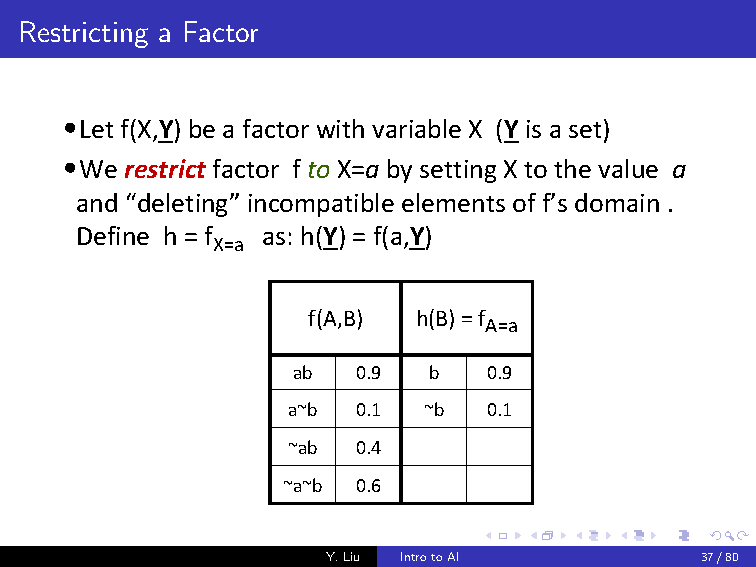
\includegraphics[width=7.5cm]{Pic/restrict}
\caption{Sumout and Restrict}
\label{Fig:sumout_restrict}
\end{figure}



\section{Codes and Results}
\subsection{Codes}
\begin{lstlisting}[language=Python,frame=single]
class VariableElimination:
    @staticmethod
    def inference(factorList, queryVariables, 
    orderedListOfHiddenVariables, evidenceList):
        for ev in evidenceList:
            #Your code here
            for i in range(len(factorList)):
                if ev in factorList[i].varList:
                    factorList[i] = factorList[i].restrict(ev, evidenceList[ev])
        for var in orderedListOfHiddenVariables:
            #Your code here
            new_factor = None
            i = 0
            while True:
                while i < len(factorList):
                    if var in factorList[i].varList:
                        if new_factor is None:
                            new_factor = factorList[i]
                        else:
                            new_factor = new_factor.multiply(factorList[i])
                        del factorList[i]
                        break
                    i += 1
                else:
                    break
            if new_factor is not None:
                factorList.append(new_factor.sumout(var))
        print "RESULT:"
        res = factorList[0]
        for factor in factorList[1:]:
            res = res.multiply(factor)
        total = sum(res.cpt.values())
        res.cpt = {k: v/total for k, v in res.cpt.items()}
        res.printInf()
    @staticmethod
    def printFactors(factorList):
        for factor in factorList:
            factor.printInf()
class Util:
    @staticmethod
    def to_binary(num, len):
        return format(num, '0' + str(len) + 'b')
class Node:
    def __init__(self, name, var_list):
        self.name = name
        self.varList = var_list
        self.cpt = {}
    def setCpt(self, cpt):
        self.cpt = cpt
    def printInf(self):
        print "Name = " + self.name
        print " vars " + str(self.varList)
        for key in self.cpt:
            print "   key: " + key + " val : " + str(self.cpt[key])
        print ""
    def multiply(self, factor):
        """function that multiplies with another factor"""
        #Your code here
        same_var = set()
        same_var_pos = list()
        for i in range(len(self.varList)):
            for j in range(len(factor.varList)):
                if self.varList[i] == factor.varList[j]:
                    same_var.add(self.varList[i])
                    same_var_pos.append((i, j))
                    break
        newList = self.varList[:]
        for var in factor.varList:
            if var not in same_var:
                newList.append(var)
        new_node = Node("f" + str(newList), newList)
        new_cpt = dict()
        for k1, v1 in self.cpt.items():
            for k2, v2 in factor.cpt.items():
                for i, j in same_var_pos:
                    if k1[i] != k2[j]:
                        break
                else:
                    new_k2 = list()
                    for i in range(len(k2)):
                        if factor.varList[i] not in same_var:
                            new_k2.append(k2[i])
                    new_cpt[k1 + ''.join(new_k2)] = v1 * v2
        new_node.setCpt(new_cpt)
        return new_node
    def sumout(self, variable):
        """function that sums out a variable given a factor"""
        #Your code here
        pos_x = self.varList.index(variable)
        new_var_list = self.varList[:pos_x] + self.varList[pos_x + 1:]
        new_node = Node("f" + str(new_var_list), new_var_list)
        new_cpt = dict()
        for k, v in self.cpt.items():
            new_k = k[:pos_x] + k[pos_x + 1:]
            if new_cpt.get(new_k) is None:
                new_cpt[new_k] = v
            else:
                new_cpt[new_k] += v
        new_node.setCpt(new_cpt)
        return new_node
    def restrict(self, variable, value):
        """function that restricts a variable to some value 
        in a given factor"""
        #Your code here
        pos_x = self.varList.index(variable)
        new_var_list = self.varList[:pos_x] + self.varList[pos_x + 1:]
        new_node = Node("f" + str(new_var_list), new_var_list)
        new_cpt = dict()
        for k, v in self.cpt.items():
            if k[pos_x] == str(value):
                new_cpt[k[:pos_x] + k[pos_x + 1:]] = v
        new_node.setCpt(new_cpt)
        return new_node
# create nodes for Bayes Net
B = Node("B", ["B"])
E = Node("E", ["E"])
A = Node("A", ["A", "B","E"])
J = Node("J", ["J", "A"])
M = Node("M", ["M", "A"])

# Generate cpt for each node
B.setCpt({'0': 0.999, '1': 0.001})
E.setCpt({'0': 0.998, '1': 0.002})
A.setCpt({'111': 0.95, '011': 0.05, '110':0.94,'010':0.06,
'101':0.29,'001':0.71,'100':0.001,'000':0.999})
J.setCpt({'11': 0.9, '01': 0.1, '10': 0.05, '00': 0.95})
M.setCpt({'11': 0.7, '01': 0.3, '10': 0.01, '00': 0.99})

print "P(A) **********************"
VariableElimination.inference([B,E,A,J,M], ['A'], ['B', 'E', 'J','M'], {})

print "P(B | J~M) **********************"
VariableElimination.inference([B,E,A,J,M], ['B'], ['E','A'], {'J':1,'M':0})
\end{lstlisting}
\subsection{Results}
\begin{figure}[h]
  \centering
  
\includegraphics[width=14cm]{result.png}
\end{figure}



%\clearpage
%\bibliography{E:/Papers/LiuLab}
%\bibliographystyle{apalike}
\end{document} 
%%% Local Variables:
%%% mode: latex
%%% TeX-master: t
%%% End:
